As a new idea, this study introduces the concept of trustless transport which replaces the need of centralized intermediation of supply and demand. We propose a mechanism which punishes hostile actors automatically resulting in no conflict resolution required from central entities. \par
In our scenario seen at figure \ref{fig:1 main overview}, we assume that the service consumer \textit{A} wants to send an physical asset to the endpoint actor \textit{B}. The third and last actor is the service provider \textit{C} who will execute the transport. Let \textit{C}, \textit{A} and \textit{B} all have an ECDSA key pair \(\{PubK_n, PrivK_n\}\) and address \(Adr_n\). \par
The scenario starts of with \textit{A} creating a request for transport minimally containing B public key, B location and A location \(\{PubK_b, Loc_b, Loc_a\}\). This request is accepted by \textit{C} which then signs \(\{PubK_c, PrivK_c\}\) a UTXO, denoted by \textit{tx1}, containing the assets equivalent cost or more to the 2/2 multisignature address of \(\{PubK_b, PubK_c\}\) denoted by \(MSig_{bc}^{n/2}\). \par

\begin{figure}[h]
\centering
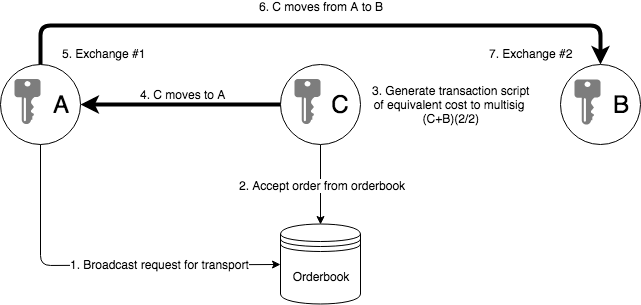
\includegraphics[width=1\textwidth]{images/main.png}
\caption{Overview test scenario}
\label{fig:1 main overview}
\end{figure}

Upon accepting \textit{C} moves to the physical location of \textit{A} bringing transaction script \textit{tx1}. As illustrated with figure \ref{fig:2 first exchange}, upon \textit{C} arriving at \textit{A} the first exchange can take place. \par

\begin{enumerate}
  \item \textit{C} innitiates the exchange by giving \textit{A} the transaction script \textit{tx1}
  \item \textit{A} generates and signs \textit{\{PubKa, PrivKa\}} UTXO \textit{tx2} containing the transporting cost of the physical asset to \(MSig_{bc}\)
  \item \textit{A} can now broadcast \textit{tx1}, \textit{tx2}
  \item \textit{A} broadcasts the ownership change of the digital asset from \textit{A $\rightarrow$ C}
  \item Wait block confirmation containing \textit{tx1} and \textit{tx2}
  \item Exchange the physical asset from \textit{A $\rightarrow$ C}.
\end{enumerate}

% \textit{C} innitiates the exchange by giving \textit{A} the transaction script of \textit{tx1}. Upon receiving the transaction script \textit{A} generates and signs \textit{\{PubKa, PrivKa\}} UTXO \textit{tx2} containing the transporting cost \textit{tc} of the physical asset to \(MSig_{bc}\). \textit{A} can now broadcast \textit{tx1}, \textit{tx2} and broadcast the ownership change of the digital asset from \textit{A $\rightarrow$ C}.
Before \textit{tx1} and \textit{tx2} get broadcasted \textit{A $\lor$ C} can individually verify if the signed transactions actually contain what they should.
% After waiting the appropiate confirmations the physical asset gets exchanged from \textit{A $\rightarrow$ C}.

\begin{figure}[h]
\centering
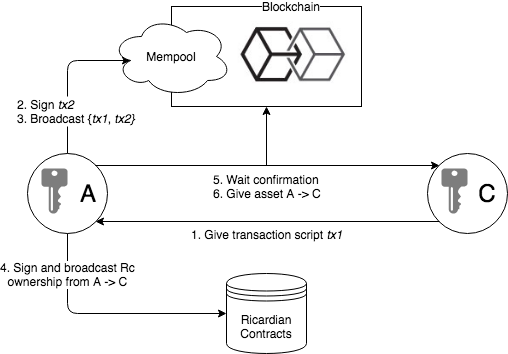
\includegraphics[width=0.8\textwidth]{images/exchange_01.png}
\caption{Exchange between A and C}
\label{fig:2 first exchange}
\end{figure}

 When \textit{C} recieves the asset he is the custodian and will move the asset to the endpoint \(Loc_b\). As illustarted with figure \ref{fig:3 dropoff exchange}, upon \textit{C} arriving at \(Loc_b\) the physical asset dropoff exchange takes place which consist out of the following steps:

\begin{enumerate}
  \item \textit{B} signs \(\{PubK_b, PrivK_b\} \rightarrow MSig_{bc}^{1/2}\) the two previously send UTXO's \textit{\{tx1, tx2\}} containing \textit{\{equivalent cost + transport cost\}} to the address of \textit{C} \(Adr_c\) and gives this transaction script to \textit{C}.
  \item Exchange physical asset \textit{C $\rightarrow$ B}
\end{enumerate}

\begin{figure}[h]
\centering
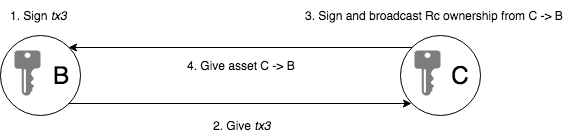
\includegraphics[width=0.6\textwidth]{images/exchange_02.png}
\caption{Exchange between C and B}
\label{fig:3 dropoff exchange}
\end{figure}

At the end of the second exchange actor \textit{C} now owns the transaction script containing \textit{\{ec+tc\}} of \(MSig_{bc}^{1/2}\) to be send to \(Adr_c\) and can sign the transaction with his own keypair whenever he wants to redeem the funds \(\{PubK_c, PrivK_c\} \rightarrow MSig_{bc}^{2/2}\).
